\documentclass[twoside]{book}

% Packages required by doxygen
\usepackage{fixltx2e}
\usepackage{calc}
\usepackage{doxygen}
\usepackage[export]{adjustbox} % also loads graphicx
\usepackage{graphicx}
\usepackage[utf8]{inputenc}
\usepackage{makeidx}
\usepackage{multicol}
\usepackage{multirow}
\PassOptionsToPackage{warn}{textcomp}
\usepackage{textcomp}
\usepackage[nointegrals]{wasysym}
\usepackage[table]{xcolor}

% Font selection
\usepackage[T1]{fontenc}
\usepackage[scaled=.90]{helvet}
\usepackage{courier}
\usepackage{amssymb}
\usepackage{sectsty}
\renewcommand{\familydefault}{\sfdefault}
\allsectionsfont{%
  \fontseries{bc}\selectfont%
  \color{darkgray}%
}
\renewcommand{\DoxyLabelFont}{%
  \fontseries{bc}\selectfont%
  \color{darkgray}%
}
\newcommand{\+}{\discretionary{\mbox{\scriptsize$\hookleftarrow$}}{}{}}

% Page & text layout
\usepackage{geometry}
\geometry{%
  a4paper,%
  top=2.5cm,%
  bottom=2.5cm,%
  left=2.5cm,%
  right=2.5cm%
}
\tolerance=750
\hfuzz=15pt
\hbadness=750
\setlength{\emergencystretch}{15pt}
\setlength{\parindent}{0cm}
\setlength{\parskip}{3ex plus 2ex minus 2ex}
\makeatletter
\renewcommand{\paragraph}{%
  \@startsection{paragraph}{4}{0ex}{-1.0ex}{1.0ex}{%
    \normalfont\normalsize\bfseries\SS@parafont%
  }%
}
\renewcommand{\subparagraph}{%
  \@startsection{subparagraph}{5}{0ex}{-1.0ex}{1.0ex}{%
    \normalfont\normalsize\bfseries\SS@subparafont%
  }%
}
\makeatother

% Headers & footers
\usepackage{fancyhdr}
\pagestyle{fancyplain}
\fancyhead[LE]{\fancyplain{}{\bfseries\thepage}}
\fancyhead[CE]{\fancyplain{}{}}
\fancyhead[RE]{\fancyplain{}{\bfseries\leftmark}}
\fancyhead[LO]{\fancyplain{}{\bfseries\rightmark}}
\fancyhead[CO]{\fancyplain{}{}}
\fancyhead[RO]{\fancyplain{}{\bfseries\thepage}}
\fancyfoot[LE]{\fancyplain{}{}}
\fancyfoot[CE]{\fancyplain{}{}}
\fancyfoot[RE]{\fancyplain{}{\bfseries\scriptsize Generated by Doxygen }}
\fancyfoot[LO]{\fancyplain{}{\bfseries\scriptsize Generated by Doxygen }}
\fancyfoot[CO]{\fancyplain{}{}}
\fancyfoot[RO]{\fancyplain{}{}}
\renewcommand{\footrulewidth}{0.4pt}
\renewcommand{\chaptermark}[1]{%
  \markboth{#1}{}%
}
\renewcommand{\sectionmark}[1]{%
  \markright{\thesection\ #1}%
}

% Indices & bibliography
\usepackage{natbib}
\usepackage[titles]{tocloft}
\setcounter{tocdepth}{3}
\setcounter{secnumdepth}{5}
\makeindex

% Hyperlinks (required, but should be loaded last)
\usepackage{ifpdf}
\ifpdf
  \usepackage[pdftex,pagebackref=true]{hyperref}
\else
  \usepackage[ps2pdf,pagebackref=true]{hyperref}
\fi
\hypersetup{%
  colorlinks=true,%
  linkcolor=blue,%
  citecolor=blue,%
  unicode%
}

% Custom commands
\newcommand{\clearemptydoublepage}{%
  \newpage{\pagestyle{empty}\cleardoublepage}%
}

\usepackage{caption}
\captionsetup{labelsep=space,justification=centering,font={bf},singlelinecheck=off,skip=4pt,position=top}

%===== C O N T E N T S =====

\begin{document}

% Titlepage & ToC
\hypersetup{pageanchor=false,
             bookmarksnumbered=true,
             pdfencoding=unicode
            }
\pagenumbering{alph}
\begin{titlepage}
\vspace*{7cm}
\begin{center}%
{\Large A\+IM \\[1ex]\large 0.\+1 }\\
\vspace*{1cm}
{\large Generated by Doxygen 1.8.13}\\
\end{center}
\end{titlepage}
\clearemptydoublepage
\pagenumbering{roman}
\tableofcontents
\clearemptydoublepage
\pagenumbering{arabic}
\hypersetup{pageanchor=true}

%--- Begin generated contents ---
\chapter{Hierarchical Index}
\section{Class Hierarchy}
This inheritance list is sorted roughly, but not completely, alphabetically\+:\begin{DoxyCompactList}
\item \contentsline{section}{Baryons}{\pageref{classBaryons}}{}
\begin{DoxyCompactList}
\item \contentsline{section}{Baryons\+\_\+A}{\pageref{classBaryons__A}}{}
\end{DoxyCompactList}
\item \contentsline{section}{bulge\+\_\+2p}{\pageref{structbulge__2p}}{}
\item \contentsline{section}{disk\+\_\+3p}{\pageref{structdisk__3p}}{}
\item \contentsline{section}{halo\+\_\+2p}{\pageref{structhalo__2p}}{}
\item \contentsline{section}{halo\+\_\+3p}{\pageref{structhalo__3p}}{}
\item \contentsline{section}{halo\+\_\+4p}{\pageref{structhalo__4p}}{}
\item \contentsline{section}{Parametric\+\_\+funcs}{\pageref{classParametric__funcs}}{}
\end{DoxyCompactList}

\chapter{Class Index}
\section{Class List}
Here are the classes, structs, unions and interfaces with brief descriptions\+:\begin{DoxyCompactList}
\item\contentsline{section}{\hyperlink{classBaryons}{Baryons} }{\pageref{classBaryons}}{}
\item\contentsline{section}{\hyperlink{classBaryons__A}{Baryons\+\_\+A} }{\pageref{classBaryons__A}}{}
\item\contentsline{section}{\hyperlink{structbulge__2p}{bulge\+\_\+2p} }{\pageref{structbulge__2p}}{}
\item\contentsline{section}{\hyperlink{structdisk__3p}{disk\+\_\+3p} }{\pageref{structdisk__3p}}{}
\item\contentsline{section}{\hyperlink{structhalo__2p}{halo\+\_\+2p} }{\pageref{structhalo__2p}}{}
\item\contentsline{section}{\hyperlink{structhalo__3p}{halo\+\_\+3p} }{\pageref{structhalo__3p}}{}
\item\contentsline{section}{\hyperlink{structhalo__4p}{halo\+\_\+4p} }{\pageref{structhalo__4p}}{}
\item\contentsline{section}{\hyperlink{classParametric__funcs}{Parametric\+\_\+funcs} }{\pageref{classParametric__funcs}}{}
\end{DoxyCompactList}

\chapter{Class Documentation}
\hypertarget{classBaryons}{}\section{Baryons Class Reference}
\label{classBaryons}\index{Baryons@{Baryons}}


Inheritance diagram for Baryons\+:\nopagebreak
\begin{figure}[H]
\begin{center}
\leavevmode
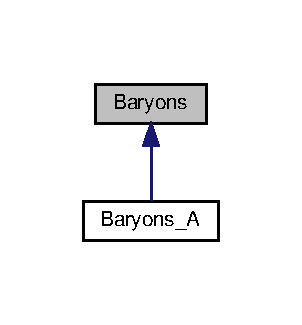
\includegraphics[width=145pt]{classBaryons__inherit__graph}
\end{center}
\end{figure}
\subsection*{Public Member Functions}
\begin{DoxyCompactItemize}
\item 
\mbox{\Hypertarget{classBaryons_afa6c0ccfacd4753da73f97858a5c94e3}\label{classBaryons_afa6c0ccfacd4753da73f97858a5c94e3}} 
virtual std\+::complex$<$ double $>$ {\bfseries psi} (std\+::complex$<$ double $>$ R2, std\+::complex$<$ double $>$ z2)=0
\item 
\mbox{\Hypertarget{classBaryons_aa0605528752cc4d3c379dccb1bb5cf06}\label{classBaryons_aa0605528752cc4d3c379dccb1bb5cf06}} 
virtual std\+::complex$<$ double $>$ {\bfseries psi\+\_\+d\+R2} (std\+::complex$<$ double $>$ R2, std\+::complex$<$ double $>$ z2)=0
\item 
\mbox{\Hypertarget{classBaryons_a91cdd21fd446a5ad96a981c670419cc6}\label{classBaryons_a91cdd21fd446a5ad96a981c670419cc6}} 
virtual std\+::complex$<$ double $>$ {\bfseries psi\+\_\+dz2} (std\+::complex$<$ double $>$ R2, std\+::complex$<$ double $>$ z2)=0
\item 
\mbox{\Hypertarget{classBaryons_a1bc5232da511f859c5bfe3b6657d4097}\label{classBaryons_a1bc5232da511f859c5bfe3b6657d4097}} 
virtual std\+::complex$<$ double $>$ {\bfseries psi\+\_\+d2\+R2} (std\+::complex$<$ double $>$ R2, std\+::complex$<$ double $>$ z2)=0
\item 
\mbox{\Hypertarget{classBaryons_af168376fa16aa35bdb0852bbf5ed4c8c}\label{classBaryons_af168376fa16aa35bdb0852bbf5ed4c8c}} 
virtual std\+::complex$<$ double $>$ {\bfseries psi\+\_\+d2z2} (std\+::complex$<$ double $>$ R2, std\+::complex$<$ double $>$ z2)=0
\end{DoxyCompactItemize}


The documentation for this class was generated from the following file\+:\begin{DoxyCompactItemize}
\item 
Baryons.\+hpp\end{DoxyCompactItemize}

\hypertarget{classBaryons__A}{}\section{Baryons\+\_\+A Class Reference}
\label{classBaryons__A}\index{Baryons\+\_\+A@{Baryons\+\_\+A}}


Inheritance diagram for Baryons\+\_\+A\+:\nopagebreak
\begin{figure}[H]
\begin{center}
\leavevmode
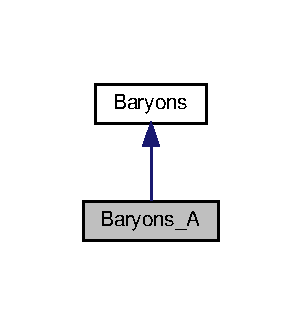
\includegraphics[width=145pt]{classBaryons__A__inherit__graph}
\end{center}
\end{figure}


Collaboration diagram for Baryons\+\_\+A\+:\nopagebreak
\begin{figure}[H]
\begin{center}
\leavevmode
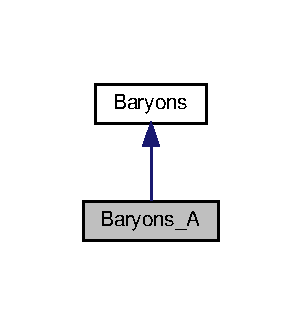
\includegraphics[width=145pt]{classBaryons__A__coll__graph}
\end{center}
\end{figure}
\subsection*{Public Member Functions}
\begin{DoxyCompactItemize}
\item 
\mbox{\Hypertarget{classBaryons__A_aa8aaefeb549270069dc70609baf120c6}\label{classBaryons__A_aa8aaefeb549270069dc70609baf120c6}} 
{\bfseries Baryons\+\_\+A} (const \hyperlink{structdisk__3p}{disk\+\_\+3p} \&M\+N1, const \hyperlink{structdisk__3p}{disk\+\_\+3p} \&M\+N2, const \hyperlink{structbulge__2p}{bulge\+\_\+2p} \&H)
\item 
\mbox{\Hypertarget{classBaryons__A_a55bbcf0080e00ea1cfb8677095c66cd7}\label{classBaryons__A_a55bbcf0080e00ea1cfb8677095c66cd7}} 
std\+::complex$<$ double $>$ {\bfseries psi} (std\+::complex$<$ double $>$ R2, std\+::complex$<$ double $>$ z2) override
\item 
\mbox{\Hypertarget{classBaryons__A_a27b009b4504623801857cdb34abd53d9}\label{classBaryons__A_a27b009b4504623801857cdb34abd53d9}} 
std\+::complex$<$ double $>$ {\bfseries psi\+\_\+d\+R2} (std\+::complex$<$ double $>$ R2, std\+::complex$<$ double $>$ z2) override
\item 
\mbox{\Hypertarget{classBaryons__A_a56a5fd239324b130fe6f254e396ae114}\label{classBaryons__A_a56a5fd239324b130fe6f254e396ae114}} 
std\+::complex$<$ double $>$ {\bfseries psi\+\_\+dz2} (std\+::complex$<$ double $>$ R2, std\+::complex$<$ double $>$ z2) override
\item 
\mbox{\Hypertarget{classBaryons__A_ac11e79381c117e51b18440c9fb638b21}\label{classBaryons__A_ac11e79381c117e51b18440c9fb638b21}} 
std\+::complex$<$ double $>$ {\bfseries psi\+\_\+d2\+R2} (std\+::complex$<$ double $>$ R2, std\+::complex$<$ double $>$ z2) override
\item 
\mbox{\Hypertarget{classBaryons__A_a168cdc73e42dda57d1e112a588c2e24d}\label{classBaryons__A_a168cdc73e42dda57d1e112a588c2e24d}} 
std\+::complex$<$ double $>$ {\bfseries psi\+\_\+d2z2} (std\+::complex$<$ double $>$ R2, std\+::complex$<$ double $>$ z2) override
\end{DoxyCompactItemize}


The documentation for this class was generated from the following files\+:\begin{DoxyCompactItemize}
\item 
Baryons\+\_\+\+A.\+hpp\item 
Baryons\+\_\+\+A.\+cpp\end{DoxyCompactItemize}

\hypertarget{structbulge__2p}{}\section{bulge\+\_\+2p Struct Reference}
\label{structbulge__2p}\index{bulge\+\_\+2p@{bulge\+\_\+2p}}


{\ttfamily \#include $<$Structs.\+hpp$>$}

\subsection*{Public Attributes}
\begin{DoxyCompactItemize}
\item 
\mbox{\Hypertarget{structbulge__2p_a9aa359566f33482bdc1b80a725ad7003}\label{structbulge__2p_a9aa359566f33482bdc1b80a725ad7003}} 
double {\bfseries M}
\item 
\mbox{\Hypertarget{structbulge__2p_acea943134cdc4383146793ff1c50d487}\label{structbulge__2p_acea943134cdc4383146793ff1c50d487}} 
double {\bfseries a}
\end{DoxyCompactItemize}


\subsection{Detailed Description}
Struct for two-\/parameter bulge 
\begin{DoxyParams}{Parameters}
{\em M} & Mass of the bulge \\
\hline
{\em a} & Scale parameter of the bulge \\
\hline
\end{DoxyParams}


The documentation for this struct was generated from the following file\+:\begin{DoxyCompactItemize}
\item 
Structs.\+hpp\end{DoxyCompactItemize}

\hypertarget{structdisk__3p}{}\section{disk\+\_\+3p Struct Reference}
\label{structdisk__3p}\index{disk\+\_\+3p@{disk\+\_\+3p}}
\subsection*{Public Attributes}
\begin{DoxyCompactItemize}
\item 
\mbox{\Hypertarget{structdisk__3p_a174f7ed754acf7215bf1f23a3f7850f6}\label{structdisk__3p_a174f7ed754acf7215bf1f23a3f7850f6}} 
double {\bfseries M}
\item 
\mbox{\Hypertarget{structdisk__3p_a99935aa770118ca0dc121fd64fddb413}\label{structdisk__3p_a99935aa770118ca0dc121fd64fddb413}} 
double {\bfseries a}
\item 
\mbox{\Hypertarget{structdisk__3p_a70dd27fdb6fee354643cb4b5b26a089d}\label{structdisk__3p_a70dd27fdb6fee354643cb4b5b26a089d}} 
double {\bfseries b}
\end{DoxyCompactItemize}


The documentation for this struct was generated from the following file\+:\begin{DoxyCompactItemize}
\item 
Structs.\+hpp\end{DoxyCompactItemize}

\hypertarget{structhalo__2p}{}\section{halo\+\_\+2p Struct Reference}
\label{structhalo__2p}\index{halo\+\_\+2p@{halo\+\_\+2p}}
\subsection*{Public Attributes}
\begin{DoxyCompactItemize}
\item 
\mbox{\Hypertarget{structhalo__2p_adc435ec1a05f25ce7e5838cd78488e9a}\label{structhalo__2p_adc435ec1a05f25ce7e5838cd78488e9a}} 
double {\bfseries rho\+\_\+s}
\item 
\mbox{\Hypertarget{structhalo__2p_ae39948a26326083311108214b1ba7cd5}\label{structhalo__2p_ae39948a26326083311108214b1ba7cd5}} 
double {\bfseries r\+\_\+s}
\end{DoxyCompactItemize}


The documentation for this struct was generated from the following file\+:\begin{DoxyCompactItemize}
\item 
Structs.\+hpp\end{DoxyCompactItemize}

\hypertarget{structhalo__3p}{}\section{halo\+\_\+3p Struct Reference}
\label{structhalo__3p}\index{halo\+\_\+3p@{halo\+\_\+3p}}


{\ttfamily \#include $<$Structs.\+hpp$>$}

\subsection*{Public Attributes}
\begin{DoxyCompactItemize}
\item 
\mbox{\Hypertarget{structhalo__3p_a9423e706c526a63b249c9b5059ee8be4}\label{structhalo__3p_a9423e706c526a63b249c9b5059ee8be4}} 
double {\bfseries rho\+\_\+s}
\item 
\mbox{\Hypertarget{structhalo__3p_a3a546f100719cca22e75271c01eece78}\label{structhalo__3p_a3a546f100719cca22e75271c01eece78}} 
double {\bfseries r\+\_\+s}
\item 
\mbox{\Hypertarget{structhalo__3p_a53b227983af0843c72d8c56aa50be08f}\label{structhalo__3p_a53b227983af0843c72d8c56aa50be08f}} 
double {\bfseries gamma}
\end{DoxyCompactItemize}


\subsection{Detailed Description}
Struct for three-\/parameter halo density profile. 
\begin{DoxyParams}{Parameters}
{\em rho\+\_\+s} & Scale density of the halo \\
\hline
{\em r\+\_\+s} & Scale radius of the halo \\
\hline
{\em gamma} & Central density slope of the halo \\
\hline
\end{DoxyParams}


The documentation for this struct was generated from the following file\+:\begin{DoxyCompactItemize}
\item 
Structs.\+hpp\end{DoxyCompactItemize}

\hypertarget{structhalo__4p}{}\section{halo\+\_\+4p Struct Reference}
\label{structhalo__4p}\index{halo\+\_\+4p@{halo\+\_\+4p}}


{\ttfamily \#include $<$Structs.\+hpp$>$}

\subsection*{Public Attributes}
\begin{DoxyCompactItemize}
\item 
\mbox{\Hypertarget{structhalo__4p_a174a0b98a3c671793ea2f7591f14bd55}\label{structhalo__4p_a174a0b98a3c671793ea2f7591f14bd55}} 
double {\bfseries rho\+\_\+s}
\item 
\mbox{\Hypertarget{structhalo__4p_aaf669aa374232d2b3aa76d7814171c77}\label{structhalo__4p_aaf669aa374232d2b3aa76d7814171c77}} 
double {\bfseries r\+\_\+s}
\item 
\mbox{\Hypertarget{structhalo__4p_aa6e000d6c31701d2ed2d76b08e9fa7f9}\label{structhalo__4p_aa6e000d6c31701d2ed2d76b08e9fa7f9}} 
double {\bfseries gamma}
\item 
\mbox{\Hypertarget{structhalo__4p_aa7de722d31c2b128e25a2979f9829232}\label{structhalo__4p_aa7de722d31c2b128e25a2979f9829232}} 
double {\bfseries q}
\end{DoxyCompactItemize}


\subsection{Detailed Description}
Struct for four-\/parameter halo density profile. 
\begin{DoxyParams}{Parameters}
{\em rho\+\_\+s} & Scale density of the halo \\
\hline
{\em r\+\_\+s} & Scale radius of the halo \\
\hline
{\em gamma} & Central density slope of the halo \\
\hline
{\em q} & Flattening of the halo along the axis of symmetry \\
\hline
\end{DoxyParams}


The documentation for this struct was generated from the following file\+:\begin{DoxyCompactItemize}
\item 
Structs.\+hpp\end{DoxyCompactItemize}

\hypertarget{classParametric__funcs}{}\section{Parametric\+\_\+funcs Class Reference}
\label{classParametric__funcs}\index{Parametric\+\_\+funcs@{Parametric\+\_\+funcs}}
\subsection*{Static Public Member Functions}
\begin{DoxyCompactItemize}
\item 
\mbox{\Hypertarget{classParametric__funcs_a63fbb6aed4d72b75e8136365805404f6}\label{classParametric__funcs_a63fbb6aed4d72b75e8136365805404f6}} 
static std\+::complex$<$ double $>$ {\bfseries psi\+\_\+\+MN} (std\+::complex$<$ double $>$ R2, std\+::complex$<$ double $>$ z2, const struct \hyperlink{structdisk__3p}{disk\+\_\+3p} \&)
\item 
\mbox{\Hypertarget{classParametric__funcs_a9835569f87964f0dad32a23d6a43a387}\label{classParametric__funcs_a9835569f87964f0dad32a23d6a43a387}} 
static std\+::complex$<$ double $>$ {\bfseries psi\+\_\+\+M\+N\+\_\+d\+R2} (std\+::complex$<$ double $>$ R2, std\+::complex$<$ double $>$ z2, const struct \hyperlink{structdisk__3p}{disk\+\_\+3p} \&)
\item 
\mbox{\Hypertarget{classParametric__funcs_a2bea359cc13f4f6beecdf0b1da8de868}\label{classParametric__funcs_a2bea359cc13f4f6beecdf0b1da8de868}} 
static std\+::complex$<$ double $>$ {\bfseries psi\+\_\+\+M\+N\+\_\+dz2} (std\+::complex$<$ double $>$ R2, std\+::complex$<$ double $>$ z2, const struct \hyperlink{structdisk__3p}{disk\+\_\+3p} \&)
\item 
\mbox{\Hypertarget{classParametric__funcs_afa840a39017db2163e9330f983e1558b}\label{classParametric__funcs_afa840a39017db2163e9330f983e1558b}} 
static std\+::complex$<$ double $>$ {\bfseries psi\+\_\+\+M\+N\+\_\+d2z2} (std\+::complex$<$ double $>$ R2, std\+::complex$<$ double $>$ z2, const struct \hyperlink{structdisk__3p}{disk\+\_\+3p} \&)
\item 
\mbox{\Hypertarget{classParametric__funcs_a92016aa86c23afb7aaa99f0bdf466962}\label{classParametric__funcs_a92016aa86c23afb7aaa99f0bdf466962}} 
static std\+::complex$<$ double $>$ {\bfseries psi\+\_\+\+M\+N\+\_\+d2\+R2z2} (std\+::complex$<$ double $>$ R2, std\+::complex$<$ double $>$ z2, const struct \hyperlink{structdisk__3p}{disk\+\_\+3p} \&)
\item 
\mbox{\Hypertarget{classParametric__funcs_a4ef64b9bbc8c109f4e3986bb425342f3}\label{classParametric__funcs_a4ef64b9bbc8c109f4e3986bb425342f3}} 
static std\+::complex$<$ double $>$ {\bfseries psi\+\_\+H} (std\+::complex$<$ double $>$ r, const struct \hyperlink{structbulge__2p}{bulge\+\_\+2p} \&)
\item 
\mbox{\Hypertarget{classParametric__funcs_ab02a5302fd6db1539e4a29d430370380}\label{classParametric__funcs_ab02a5302fd6db1539e4a29d430370380}} 
static std\+::complex$<$ double $>$ {\bfseries psi\+\_\+\+H\+\_\+dr2} (std\+::complex$<$ double $>$ r, const struct \hyperlink{structbulge__2p}{bulge\+\_\+2p} \&)
\item 
\mbox{\Hypertarget{classParametric__funcs_a8e663fb60e664f232a5779dc107782a6}\label{classParametric__funcs_a8e663fb60e664f232a5779dc107782a6}} 
static std\+::complex$<$ double $>$ {\bfseries psi\+\_\+\+H\+\_\+d2r2} (std\+::complex$<$ double $>$ r, const struct \hyperlink{structbulge__2p}{bulge\+\_\+2p} \&)
\end{DoxyCompactItemize}


The documentation for this class was generated from the following files\+:\begin{DoxyCompactItemize}
\item 
Parametric\+\_\+funcs.\+hpp\item 
Parametric\+\_\+funcs.\+cpp\end{DoxyCompactItemize}

%--- End generated contents ---

% Index
\backmatter
\newpage
\phantomsection
\clearemptydoublepage
\addcontentsline{toc}{chapter}{Index}
\printindex

\end{document}
